\section{Results}\label{sec:results}
\subsection{A compact operating point}
Table~\ref{tab:main} reports the primary result and separates it from published context. Across three training seeds, the 160-pixel model achieves 59.0$\pm$0.1\% target \pacc{0.5}, 31.5$\pm$0.4\% \pacc{0.7}, and 52.9$\pm$0.4\% mIoU (sample standard deviations). The seed-42 checkpoint reaches 58.9\% \pacc{0.5} and 53.3\% mIoU; we retain it as the reference rather than selecting a seed using test performance. Its hand \pacc{0.5} is 92.6\%, and mean fingertip error is 3.89 pixels at the 160-pixel input. Accurate hand and fingertip estimates coexist with a much larger target-localisation error.

\begin{table*}[t]
\centering
\caption{Target localisation and model scale. Accuracy entries are percentages. Our rows use all 2,604 target-positive test images; \emph{large gap} is \pacc{0.5} on the 209 images with normalised fingertip--box gap $>0.08$. Published values are contextual, not a controlled ranking: $^\ddagger$~PointVG-R~\cite{li2026pointvgr}, Table~1, uses the EgoPoint-CoT setting and does not explicitly specify no-target scoring; $^\dagger$~EgoPoint-Ground~\cite{egopoint}, Table~4, uses pointing-only grounding with a supplied hand box and an unstated evaluated subset. Published thresholds may use $>$ rather than our $\geq$. Dashes mean not reported or not applicable. Latency is the recorded glasses inference range for the 160-pixel model only.}
\label{tab:main}
\footnotesize
\setlength{\tabcolsep}{4pt}
\begin{tabular}{lrrrrrrr}
\toprule
Method / setting & Params & \pacc{0.3} & \pacc{0.5} & \pacc{0.7} & mIoU & Large gap & Latency\\
\midrule
\multicolumn{8}{l}{\emph{Published, trained on EgoPoint (not rerun)}}\\
PointVG-R$^\ddagger$, image + instruction, SFT + RL & 7B & 88.1 & 83.6 & 74.5 & 75.7 & -- & --\\
Qwen2.5-VL-7B$^\ddagger$, image + instruction, SFT & 7B & 68.7 & 63.6 & 56.7 & 59.8 & -- & --\\
\multicolumn{8}{l}{\emph{Published, zero-shot / inference-only (not rerun)}}\\
Qwen2.5-VL-7B$^\ddagger$, image + instruction & 7B & 54.2 & 49.8 & 42.9 & 45.5 & -- & --\\
Qwen3-VL-8B$^\ddagger$, image + instruction & 8B & 48.1 & 44.5 & 39.0 & 43.0 & -- & --\\
SV-CoT$^\dagger$, image + hand box & -- & 69.4 & 63.9 & 55.6 & -- & -- & --\\
Qwen3-VL-4B$^\dagger$, image + hand box & 4B & 67.1 & 61.2 & 53.2 & -- & -- & --\\
\midrule
\textbf{SpatialNet}, image only, seed 42 & 0.72M & 78.6 & 58.9 & 31.8 & 53.3 & 25.4 & 60--80\,ms\\
\quad mean $\pm$ sample std, three seeds & & $78.1\pm0.6$ & $59.0\pm0.1$ & $31.5\pm0.4$ & $52.9\pm0.4$ & $26.3\pm1.3$ & --\\
SpatialNet, 224 px input & 0.72M & 78.8 & 62.4 & 37.1 & 54.8 & 35.9 & --\\
SpatialNet, 320 px input & 0.72M & 79.4 & 65.1 & 40.3 & 56.5 & 34.9 & --\\
\bottomrule
\end{tabular}
\end{table*}

\paragraph{The box is more than a fingertip location.}
As a diagnostic reference, we place a box with mean training-set width and height at the \emph{ground-truth} fingertip. It reaches only 11.4\% \pacc{0.5}. This establishes that even an oracle fingertip is insufficient for this simple extent rule; it does not establish an upper bound for richer fingertip-conditioned methods. SpatialNet's gain reflects learning where the target centre lies and how far the referred object extends, not merely learning to find the finger.

\paragraph{Published accuracy context.}
PointVG-R reports substantially higher localisation under its protocol. The comparison also reveals why a single IoU threshold is insufficient: the zero-shot Qwen row is lower than SpatialNet at \pacc{0.5}, but higher at \pacc{0.7}. These observations motivate precision analysis; they do not establish relative superiority. The published works list a 3,072-image test split, while our conversion excludes 43 test positives and our target denominator excludes 425 negatives. Their no-target scoring is not explicit; the hand-box-assisted rows additionally use different inputs and an unstated subset. We therefore make no parity claim and do not construct a cross-hardware speedup ratio. The experimentally supported claim is the measured operating point of our own model.

\subsection{Resolution and image-plane separation}\label{sec:resolution}
Figure~\ref{fig:resolution} shows the clearest accuracy lever. At fixed parameter count, increasing input from 160 to 224 pixels raises \pacc{0.5} by 3.5 points (95\% paired interval [1.8, 5.1]); 320 pixels raises it by 6.2 points [4.4, 8.0], reaching 65.1\%. Stricter precision improves more: \pacc{0.7} rises from 31.8 to 37.1 and 40.3\%. Counted computation grows from 0.23 to 0.45 and 0.92 GFLOPs. Resolution therefore exchanges computation for accuracy without requiring more stored parameters.

\begin{figure*}[t]
\centering
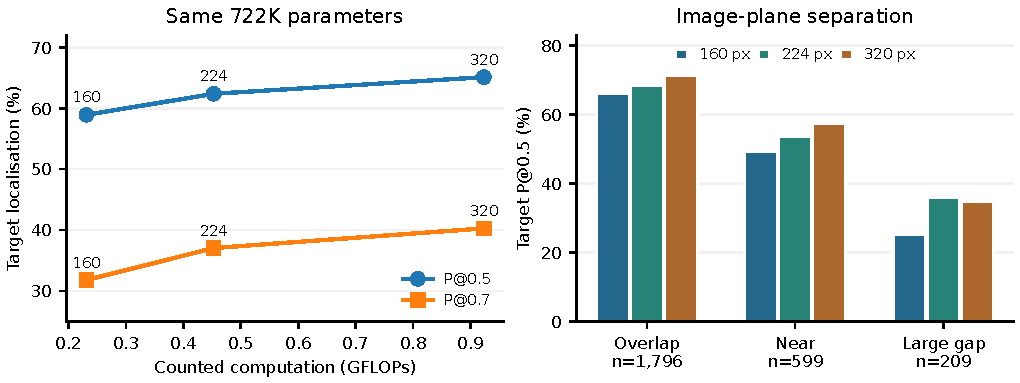
\includegraphics[width=\textwidth]{figures/resolution.pdf}
\caption{Resolution is the strongest tested accuracy lever. Left: localisation at three input sizes with the same 722K parameters; labels denote input side length. Right: \pacc{0.5} by annotated image-plane fingertip--box gap. The 320-pixel run uses source images reconverted at that resolution. Higher-resolution runs use one training seed each, and their device costs were not measured.}
\label{fig:resolution}
\end{figure*}

The strata explain what the pooled gain does and does not solve. At 160 pixels, \pacc{0.5} is 66.0\% for overlap, 49.2\% for near and 25.4\% for large-gap targets. Hand \pacc{0.5} remains approximately 93\% in all three groups. Thus, the decline cannot be explained simply by failure to find a hand. Large-gap target accuracy improves to 35.9\% at 224 pixels but is 34.9\% at 320. These single-run results show no further gain for that subset, while overall box precision continues to improve. They are consistent with unresolved reference and extent ambiguity, but do not isolate its cause or establish a resolution ceiling.

Direction also requires careful interpretation. The reference model's median angular error is 18.6 degrees against the fingertip-to-target-centre annotation. Higher resolution does not consistently reduce the mean error. Since the label itself depends on object extent, direction errors conflate geometric pointing and which target centre should be selected. Increasing spatial detail addresses part of the problem, but does not supply a separate measurement of the wearer's intended ray.

\subsection{Which design choices contribute?}\label{sec:ablation}
\begin{figure*}[t]
\centering
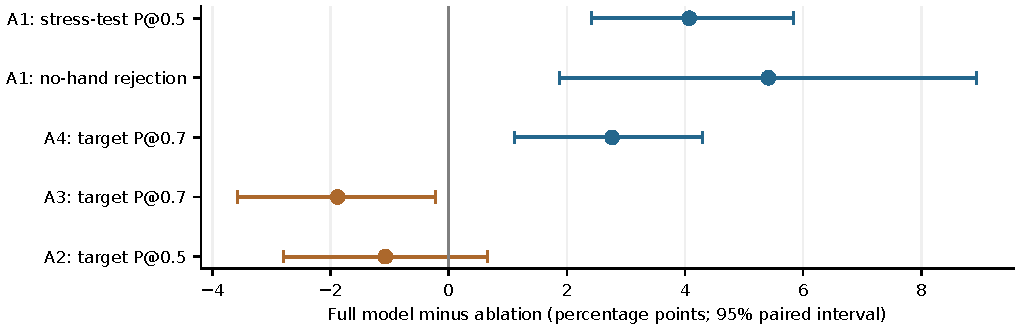
\includegraphics[width=0.93\textwidth]{figures/ablations.pdf}
\caption{Benefits are specific rather than universal. Positive values favour the full model; negative values favour removal of the component. Intervals use paired test images for the saved checkpoints, not repeated training. Distractor training helps the synthetic stress test, instance conditioning helps stricter box precision, and removing the ray branch improves that same precision metric.}
\label{fig:ablations}
\end{figure*}
Table~\ref{tab:ablations} reports every ablation's clean target \pacc{0.5} and \pacc{0.7}; Figure~\ref{fig:ablations} highlights selected mechanism-specific effects. All four changes lie within 1.1 points of the full model at \pacc{0.5}, and their paired intervals include zero. We therefore do not claim that any one component is necessary for the headline accuracy. Their differences appear in precision, auxiliary geometry and interference.

\begin{table}[t]
\centering
\caption{All four ablations, clean test set. Parameter count is in millions. A1/A2 are bundled training changes; A4 retains local box-size heads and target ray conditioning. Each variant has one training seed.}
\label{tab:ablations}
\small
\setlength{\tabcolsep}{3.5pt}
\begin{tabular}{lrrr}
\toprule
Variant & Params & \pacc{0.5} & \pacc{0.7}\\
\midrule
Full & 0.722 & 58.9 & 31.8\\
A1: no distractor training & 0.722 & 58.8 & 30.5\\
A2: no consistency losses & 0.722 & 60.0 & 32.4\\
A3: no target ray branch & 0.709 & 59.6 & 33.7\\
A4: no instance conditioning & 0.709 & 58.6 & 29.0\\
\bottomrule
\end{tabular}
\end{table}

\paragraph{Instance conditioning supports precise localisation.}
A4 reduces \pacc{0.7} by 2.8 points (full-minus-ablation interval [1.1, 4.3]) and hand mIoU by 1.8 points. Its mean direction error increases by 3.4 degrees. The reduction in target precision is larger than the 0.8-point largest \pacc{0.7} change observed between the reference and the other full-model seeds. This supports instance conditioning as a useful inductive bias under the tested recipe. It does not prove that every part of the bundled pathway is needed. A4 selected epoch 54 rather than 100, so the effect includes the training trajectory induced by that intervention.

Small targets provide supporting, less stable evidence. For boxes occupying less than 3\% of image area ($n=309$), \pacc{0.5} falls from 36.9 to 25.6\% in A4. However, the full-model seeds span 27.8--36.9\%, making this metric much more training-sensitive than the headline score. We accordingly place greater weight on the broader high-IoU and hand-box results.

\paragraph{Better direction does not imply a better target box.}
A2 removes both geometric consistency losses. Large-gap mean direction error increases by 5.6 degrees [2.1, 9.4], yet target \pacc{0.5} does not decline. This establishes a separation between improving the supervised direction and using that improvement for localisation. It provides no evidence that these losses improve the target box.

A3 offers stronger counterevidence to the original ray-conditioning hypothesis. Retraining without the target ray branch yields 59.6\% \pacc{0.5} and improves \pacc{0.7} by 1.9 points [0.2, 3.6]. The branch therefore earns no accuracy claim here. A3 selects a later checkpoint (epoch 120), and only one retraining is available, so the result should not be generalised into a universal claim against geometry.

Diagnostic interventions help interpret this outcome. On a fixed test subset, removing the branch \emph{only at inference} lowers localisation in the full trained model, whereas retraining A3 compensates for its absence. Spatial probes of the learned branch show a stronger association with proximity to the fingertip than with the signed forward ray coordinate. These findings are consistent with a proximity cue that the visual pathway can also learn. They do not prove that dataset imbalance caused this behaviour: the conditioning branch also receives appearance features, and the probe is observational. The 69\% overlap prevalence makes this a plausible explanation to investigate, not a demonstrated causal mechanism.



\subsection{Synthetic hand interference}
A1 isolates the combined effect of distractor pasting and its heatmap-negative weighting. In the synthetic stress condition, the full model reaches 60.1\% target \pacc{0.5}, compared with 56.1\% without this training. The 4.1-point paired difference has interval [2.4, 5.8]. On the 425 no-wearer-hand frames containing pasted hands, correct rejection improves from 86.4 to 91.8\%, a 5.4-point difference [1.9, 8.9]. The clean \pacc{0.5} difference is only 0.1 point, with an interval crossing zero. These results support robustness to the tested interference without a detected clean accuracy penalty.

Two cautions constrain this conclusion. First, a higher stress-test score than clean score does not mean other hands intrinsically help localisation; the transformation changes the image, and its clean-to-stress contrast is not the controlled training intervention. Second, A4 shows no clear ownership deterioration, so the evidence attributes synthetic robustness to the distractor-training package, not necessarily to instance-conditioned gates. The limited crop positions and shared train/test augmentation family also allow positional shortcuts. Real multi-hand generalisation remains unestablished.

\begin{quote}\begin{minipage}{\linewidth}\small
\tFive{Insert the real smart-glasses multi-hand check here: participant/frame counts and capture conditions; consent or ethics status and image-retention policy; wearer/target annotation and handling of disagreements; target localisation and no-wearer-hand rejection with denominators and uncertainty; and representative successes and failures. Distinguish repeated frames from independent scenes. Replace this block with the observed results and update the corresponding scope statements. No real multi-hand result is claimed in this version.}
\end{minipage}\end{quote}

\begin{figure*}[t]
\centering
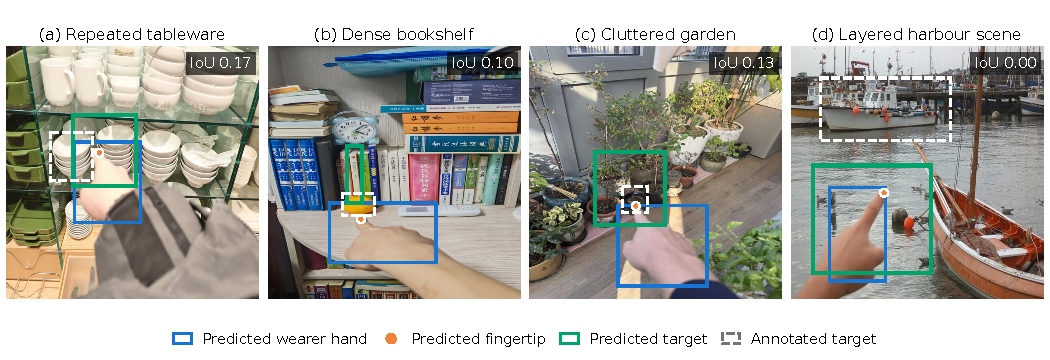
\includegraphics[width=\textwidth]{figures/qualitative.pdf}
\caption{Selected complex failures of the 722K-parameter model. Repeated tableware and dense books create neighbouring-instance ambiguity (a,b); foliage and small objects complicate target extent (c); several depth layers separate the fingertip from the labelled boat (d). Colours match Figure~\ref{fig:teaser}. Predictions and IoUs are from the saved test evaluation. These are deliberately selected hard cases, not evidence that failures occur only in complex scenes.}
\label{fig:qualitative}
\end{figure*}
\subsection{Prototype execution on smart glasses}
The 160-pixel checkpoint was deployed on a pre-production glasses unit with an onboard camera and local inference capability. The recorded engineering observations give 60--80\,ms inference per frame. This establishes execution on the prototype, but the record does not supply a latency distribution, number of repeated trials or an end-to-end timing decomposition. We therefore report the observed range rather than a percentile estimate, sustained throughput or camera-to-action response time.

The FP16 state dictionary occupies about 1.6\,MiB. A recorded additional-memory observation of approximately 100\,KB is relative to an already loaded application/model and is not total inference memory. Likewise, one-minute battery readings were 9 percentage points during continuous local inference and 16 points while streaming at 0.5 frames/s to a phone. These coarse, unmatched operating modes and the engineering power stack do not establish energy per inference, expected battery life or a general advantage over offloading. The result relevant to this paper is local feasibility at the reported latency; power and memory observations provide bounded implementation context.

\subsection{Qualitative boundary of the method}
Figure~\ref{fig:qualitative} focuses on challenging scenes with repeated objects, clutter or multiple depth layers. The tiny model selects an adjacent tableware stack or book, includes surrounding garden content, and places a foreground box instead of finding the labelled boat. These examples expose the distinction between locating a hand and resolving its reference: visual similarity and target extent remain difficult even when the hand is visible. The examples are selected to illustrate complex failures, not to estimate their prevalence or suggest that simpler scenes are error-free. Aggregate results above include every target-positive test image.


